\chapter*{Solutions to Additional Exercises}
\section*{Basic Concepts}
\begin{enumerate}
\item 
\begin{lstlisting}
>> Ts = 3;
>> T0 = 49;
>> k = 0.45;
>> t = 3;
>> T = round(Ts + (T0 - Ts) * exp(-k*t))
T =
	15
\end{lstlisting}
\subsubsection{Comments:}
\begin{itemize}
\item The \mcode{round} function rounds to the nearest integer value.
\end{itemize}

\item 
\begin{align*}
& f(t) = f(0) e^{kt}, \\
&\Leftrightarrow \frac{f(t)}{f(0)} = e^{kt}, \\
&\Leftrightarrow ln \left( \frac{f(t)}{f(0)} \right) = ln ( e^{kt} ), \\
&\Leftrightarrow k = ln \left( \frac{f(t)}{f(0)} \right) \cdot \frac{1}{t}
\end{align*}
\begin{lstlisting}
>> t = 3.261;
>> F0 = 100;
>> Ft = 50;
>> k = log(Ft/F0) * (1/t)
k = 
	-0.2126
>> t = 7;
>> Ft = F0 * exp(k*t)
Ft =
	 22.5847
\end{lstlisting}

\item
\begin{align*}
& M = \frac{2}{3} log_{10} \left( \frac{E}{E_0} \right), \\
&\Leftrightarrow \frac{3M}{2} = log_{10} \left( \frac{E}{E_0} \right), \\
&\Leftrightarrow 10^{\frac{3M}{2}} = 10^{log_{10} \left( \frac{E}{E_0} \right)}, \\
&\Leftrightarrow E = 10^{\frac{3M}{2}} \cdot E_0
\end{align*}
\begin{lstlisting}
>> E0 = 10^4.4;
>> M1 = 6.9;
>> M2 = 7.1;
>> E1 = 10^((3*M1)/2) * E0;
>> E2 = 10^((3*M2)/2) * E0;
>> Ediff = E2/E1
Ediff =
		1.9953
\end{lstlisting}

\item
\begin{lstlisting}
>> A = 16.0137;
>> B = 3096.52;
>> C = -53.67;
>> T = 315;
>> P = exp(A - B/(C + T))
P = 
	 64.3682
>> T = 405;
>> P = exp(A - B/(C + T))
P = 
	 1.3394e+03
\end{lstlisting}

\clearpage
\item
The total (equivalent) force applied to the bracket is obtained by adding the forces acting on the bracket.
\begin{itemize}
\item Write each force as a vector with two elements, where the first element is the $x$ component of the vector and the second element is the $y$ component.
\item Determine the vector form of the equivalent force by adding the vectors.
\item Determine the magnitude and direction of the equivalent force.
\end{itemize}
\begin{lstlisting}
>> F1M = 400; F2M = 500; F3M = 700;
>> theta1 = -20; theta2 = 30; theta3 = 143;
>> F1 = F1M * [cosd(theta1) sind(theta1)]
F1 =
    375.8770 -136.8081
>> F2 = F2M * [cosd(theta2) sind(theta2)]
F2 =
    433.0127  250.0000
>> F3 = F3M * [cosd(theta3) sind(theta3)]
F3 =
    -559.0449  421.2705
>> Ftot = F1 + F2 + F3
Ftot =
    249.8449  534.4625
>> FtotM = sqrt(Ftot(1)^2 + Ftot(2)^2)
FtotM =
    589.9768
>> theta = atand(Ftot(2) / Ftot(1))
theta =
    64.9453
\end{lstlisting}
\subsubsection{Comments:}
\begin{itemize}
\item On Lines 1 and 2 the magnitudes and angles to the $x$ axis of the forces are entered.
\item On Lines 3, 6 and 9 the two components ($x$ and $y$) of each force are calculated.
\item On Line 12 the three force vectors are added together.
\item Finally on Lines 15 and 18 the magnitude and angle to the $x$ axis of the total force are calculated.
\end{itemize}

\clearpage
\item
\begin{lstlisting}
>> m = [2 4 5 10 20 50];
>> F = [12.5 23.5 30 61 117 294];
>> mu = F./(m*9.81)
mu =
    0.6371    0.5989    0.6116    0.6218    0.5963    0.5994
>> mu_ave = mean(mu)
mu_ave =
    0.6109
\end{lstlisting}
\subsubsection{Comments:}
\begin{itemize}
\item On Line 6 the \mcode{mean} function is used to determine the average of the elements in the vector \mcode{mu}.
\end{itemize}

\item
The equations for the four meshes are:
\begin{align*}
& V_1 - R_1 i_1 - R_3(i_1-i_3) - R_2(i_1-i_2) = 0 \\
& -R_5 i_2 - R_2(i_2-i_1) - R_4(i_2-i_3) - R_7(i_2-i_4) = 0 \\
& -V_2 - R_6(i_3-i_4) - R_4(i_3-i_2) - R_3(i_3-i_1) = 0 \\
& V_3 - R_8 i_4 - R_7(i_4-i_2) - R_6(i_4-i_3) = 0
\end{align*}
The equations can be re-written in the matrix form $Ax = B$:
\begin{equation*}
\begin{split}
\left[ \begin{array}{cccc} -(R_1 + R_2 + R_3) & R_2 & R_3 & 0 \\ R_2 & -(R_2 + R_4 + R_5 + R_7) & R_4 & R_7 \\ R_3 & R_4 & -(R_3 + R_4 + R_6) & R_6 \\ 0 & R_7 & R_6 & -(R_6 + R_7 + R_8) \end{array} \right] \\
\cdot \left[ \begin{array}{c} i_1 \\ i_2 \\ i_3 \\ i_4 \end{array} \right] = \left[ \begin{array}{c} -V_1 \\ 0 \\ V_2 \\ -V_3 \end{array} \right]
\end{split}
\end{equation*}
\begin{lstlisting}
>> V1 = 20; V2 = 12; V3 = 40;
>> R1 = 18; R2 = 10; R3 = 16; R4 = 6;
>> R5 = 15; R6 = 8; R7 = 12; R8 = 14;
>> A = [-(R1+R2+R3) R2 R3 0;
R2 -(R2+R4+R5+R7) R4 R7;
R3 R4 -(R3+R4+R6) R6;
0 R7 R6 -(R6+R7+R8)]
A =
   -44    10    16     0
    10   -43     6    12
    16     6   -30     8
     0    12     8   -34
>> B = [-V1; 0; V2; -V3]
B =
   -20
     0
    12
   -40
>> I = A\B
I =
    0.8411
    0.7206
    0.6127
    1.5750
>> R1i = I(1)
R1i =
    0.8411
>> R2i = I(1) - I(2)
R2i =
    0.1205
>> R3i = I(1) - I(3)
R3i =
    0.2284
>> R4i = I(2) - I(3)
R4i =
    0.1079
>> R5i = I(2)
R5i =
    0.7206
>> R6i = I(4) - I(3)
R6i =
    0.9623
>> R7i = I(4) - I(2)
R7i =
    0.8543
>> R8i = I(4)
R8i =
    1.5750
\end{lstlisting}
\subsubsection{Comments:}
\begin{itemize}
\item On Line 19 the left division is used to solve a system of equations of the form $Ax = B$.
\item One Lines 21--24 the four elements of \mcode{I} are the mesh currents $i_1, i_2, i_3, i_4$.
\end{itemize}

\clearpage
\section*{Plotting}
\item
\begin{lstlisting}
>> F = [0 13345 26689 40479 42703 43592 44482 44927 45372 ...
46276 47908 49035 50265 53213 56161];
>> L = [25 25.037 25.073 25.113 25.122 25.125 25.132 25.144 ...
25.164 25.208 25.409 25.646 26.084 27.398 29.150];
>> A0 = 2*pi*6.4^2;
>> L0 = 25;
>> sig_e = F./A0;
>> eps_e = (L - L0)./L0;
>> sig_t = (F./A0) .* (L./L0);
>> eps_t = log(L./L0);
>> plot(eps_e,sig_e,eps_t,sig_t,'r'), grid on, 
xlabel('Strain'), ylabel('Stress (Pa)'), ...
legend('Engineering stress-strain','True stress-strain'), ...
title('Tensile test of an aluminium specimen')
\end{lstlisting}
\begin{figure}[h]
	\myfloatalign
	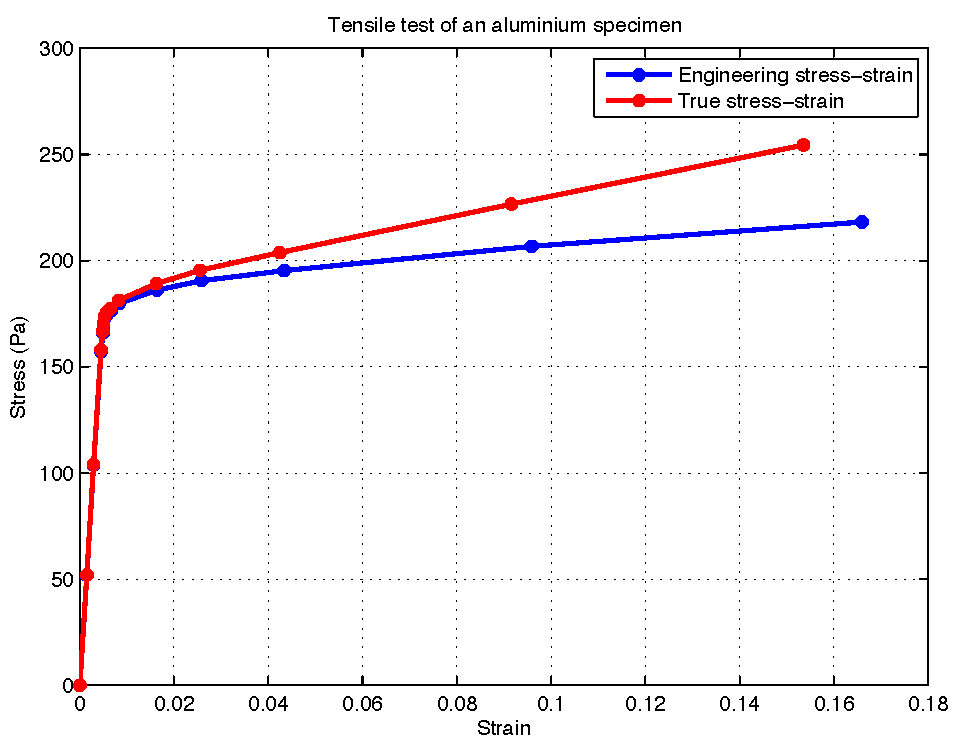
\includegraphics[width=\linewidth]{Graphics/Additional-Ex/tension-test-plot}
	\caption{Tension test of an aluminium specimen}
	\label{fig:tension-test-plot}
\end{figure}

\clearpage
\item
\begin{lstlisting}
>> R = 4; L = 1.3; V = 12;
>> t1 = linspace(0,0.5,25);
>> t2 = linspace(0.5,2,25);
>> i1 = (V/R) * (1 - exp((-R*t1)./L));
>> i2 = exp((-R*t2)./L) * (V/R) .* (exp((0.5*R)/L) - 1);
>> plot(t1,i1,'b',t2,i2,'b'), grid on, xlabel('Time (s)'), ...
ylabel('Current (A)'), title('Current in a RL circuit')
\end{lstlisting}
\begin{figure}[h]
	\myfloatalign
	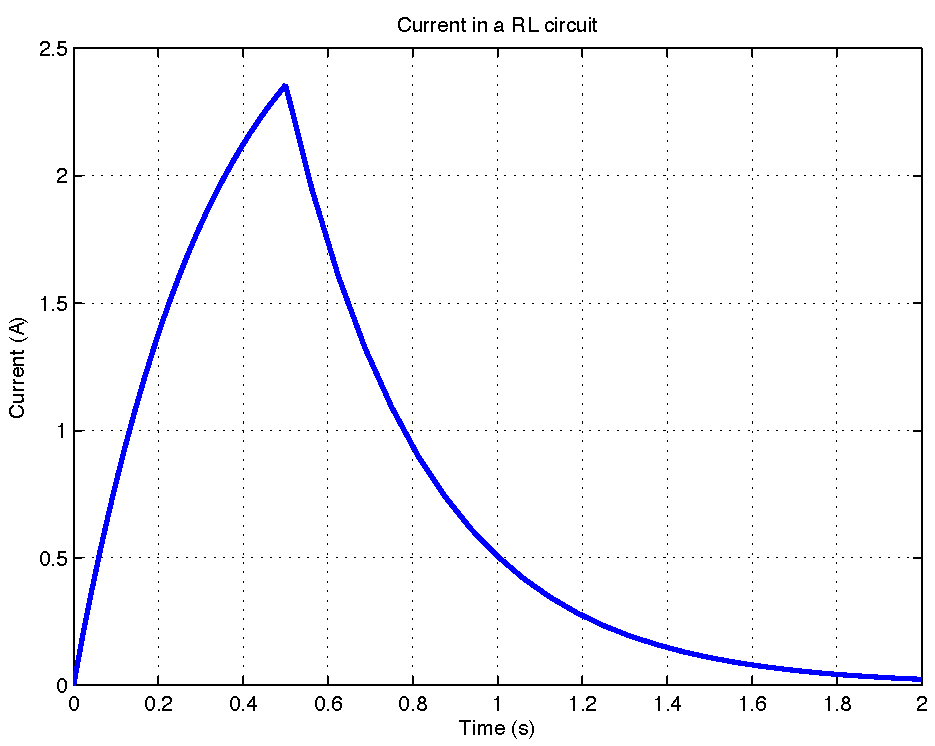
\includegraphics[width=\linewidth]{Graphics/Additional-Ex/RL-circuit-plot}
	\caption{Current in a \textit{RL} circuit}
	\label{fig:RL-circuit-plot}
\end{figure}

\clearpage
\item
\begin{lstlisting}
>> f0 = 12; wn = 10; w = 12;
>> t = linspace(0,2,50);
>> x = (2*f0) / (wn^2 - w^2) * sin(((wn - w)/2)*t) .* ...
sin(((wn - w)/2)*t);
>> plot(t,x), grid on, xlabel('Time (s)'), ...
ylabel('Amplitude'), title('Vibration of a helicopter body')
\end{lstlisting}
\begin{figure}[h]
	\myfloatalign
	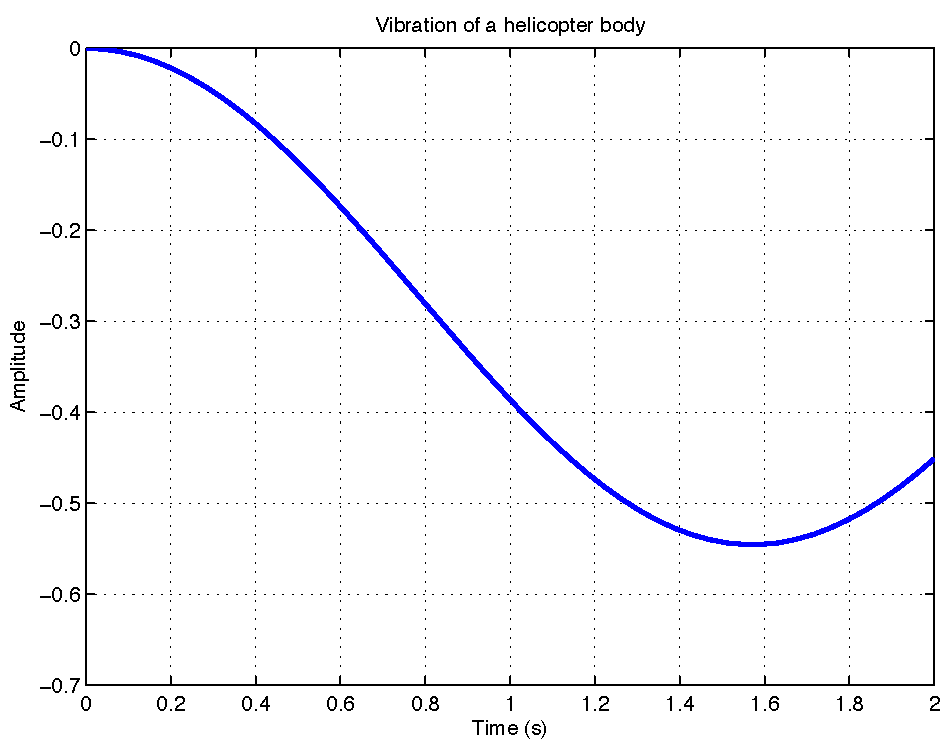
\includegraphics[width=\linewidth]{Graphics/Additional-Ex/heli-vib-plot}
	\caption{Vibration of a helicopter body}
	\label{fig:heli-vib-plot}
\end{figure}

\clearpage
\item
\begin{lstlisting}
>> n = 1; R = 0.08206; T = 300; a = 1.39; b = 0.0391;
>> V = 0.08:0.02:6;
>> P = (n*R*T) ./ (V - n*b) - (n^2 * a) ./ (V.^2);
>> id_gas_eq = (P.*V) / (R*T);
>> plot(P,id_gas_eq), grid on, xlabel('Pressure (atm)'), ...
ylabel('PV/RT'), title('Behaviour of nitrogen gas')
\end{lstlisting}
\begin{figure}[h]
	\myfloatalign
	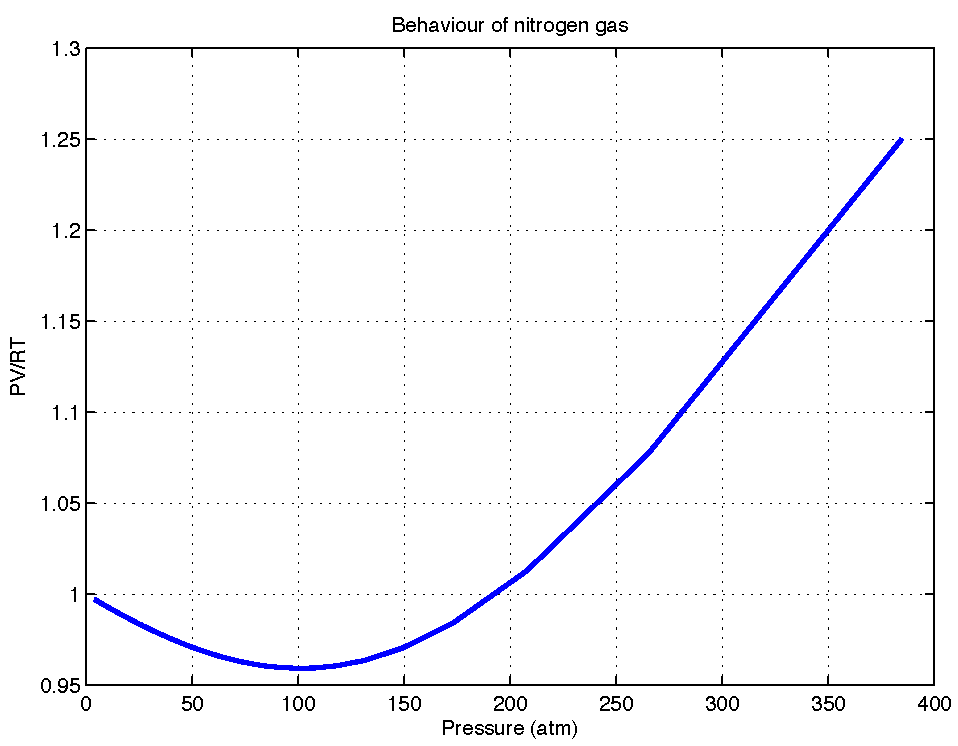
\includegraphics[width=\linewidth]{Graphics/Additional-Ex/nitrogen-plot}
	\caption{Behaviour of nitrogen gas}
	\label{fig:nitrogen-plot}
\end{figure}
The ideal gas equation is a linear function. The plot of $P$ vs. $\frac{PV}{RT}$ for nitrogen shows that it is not a linear function and therefore does not obey the ideal gas equation.

\clearpage
\item
\begin{lstlisting}
>> L = 20; E = 200E9; I = 348E-6; w = 5E3;
>> x1 = linspace(0,(2/3)*L,50);
>> x2 = linspace((2/3)*L,L,50);
>> y1 = ((-w*x1) ./ (24*L*E*I)) .* ...
(L*x1.^3 - (16/9)*L^2*x1.^2 + (64/81)*L.^4);
>> y2 = ((-w*L) ./ (54*E*I)) .* ...
(2*x2.^3 - 6*L*x2.^2 + (40/9)*L^2.*x2 - (4/9)*L^3);
>> plot(x1,y1,'b',x2,y2,'b'), grid on, ...
xlabel('x (m)'), ylabel('Deflection y (m)'), ...
title('Deflection of a steel beam')
\end{lstlisting}
\begin{figure}[h]
	\myfloatalign
	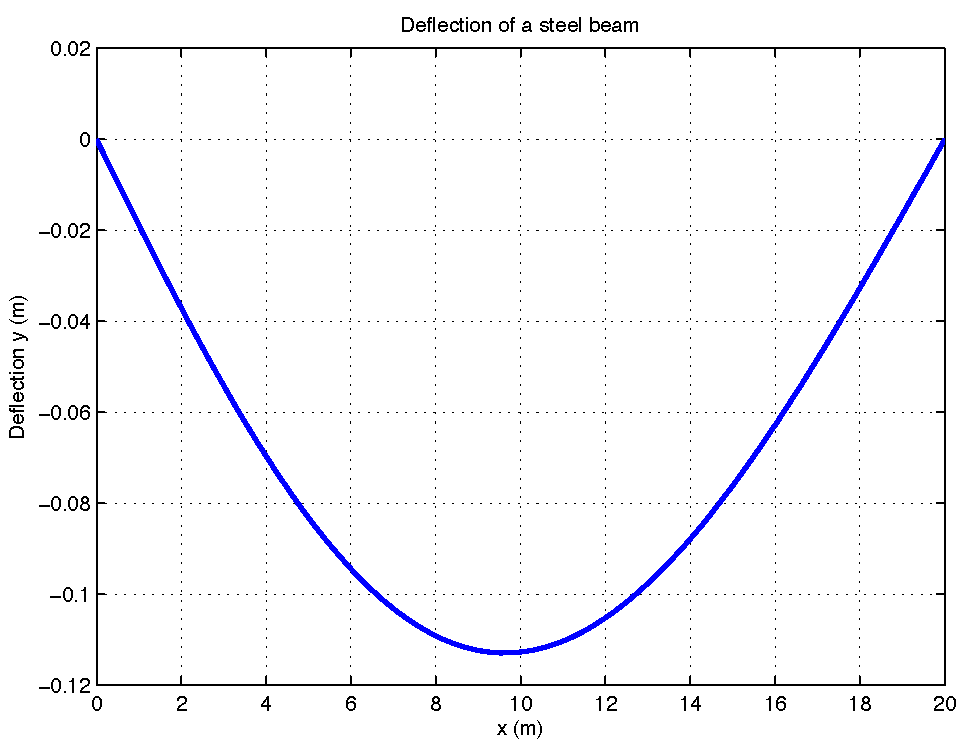
\includegraphics[width=\linewidth]{Graphics/Additional-Ex/steel-beam-plot}
	\caption{Deflection of a steel beam}
	\label{fig:steel-beam-plot}
\end{figure}

\clearpage
\item
\begin{lstlisting}
>> x = -50:5:50; y = x; k = 0.254;
>> [xx, yy] = meshgrid(x,y);
>> w = k * (xx.^2 - yy.^2);
>> surf(xx,yy,w), colorbar, xlabel('x (mm)'), ...
ylabel('y (mm)'), zlabel('Deflection (mm)'), ...
title('Deflection of a composite plate')
\end{lstlisting}
\begin{figure}[h]
	\myfloatalign
	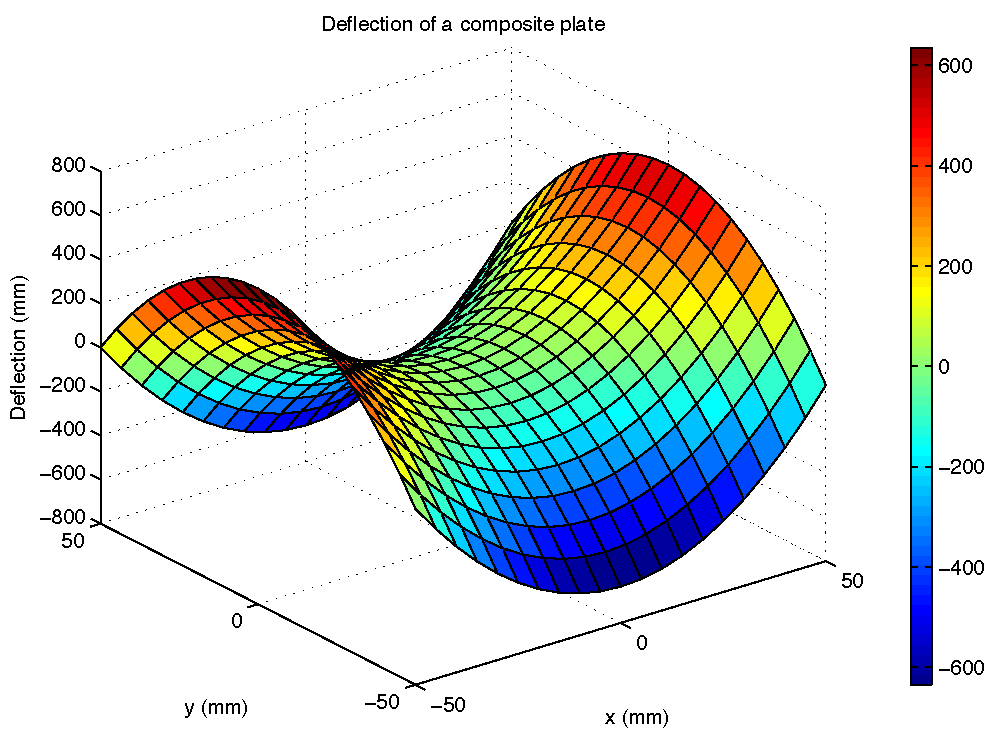
\includegraphics[width=\linewidth]{Graphics/Additional-Ex/3D-plate-deflection-plot}
	\caption{Deflection of a composite plate}
	\label{fig:3D-plate-deflection-plot}
\end{figure}

\clearpage
\item
\begin{lstlisting}
>> n = 1.5; R = 0.08206; a = 1.39; b = 0.03913;
>> V = linspace(0.3,1.2,25);
>> T = linspace(273,473,25);
>> [VV, TT] = meshgrid(V,T);
>> P = ((n*R*TT) ./ (VV-b)) - ((n^2*a) ./ VV.^2);
>> surf(VV,TT,P), colorbar, xlabel('Volume (L)'), ...
ylabel('Temperature (K)'), zlabel('Pressure (atm)'), ...
title('van der Waals equation for nitrogen gas')
\end{lstlisting}
\begin{figure}[h]
	\myfloatalign
	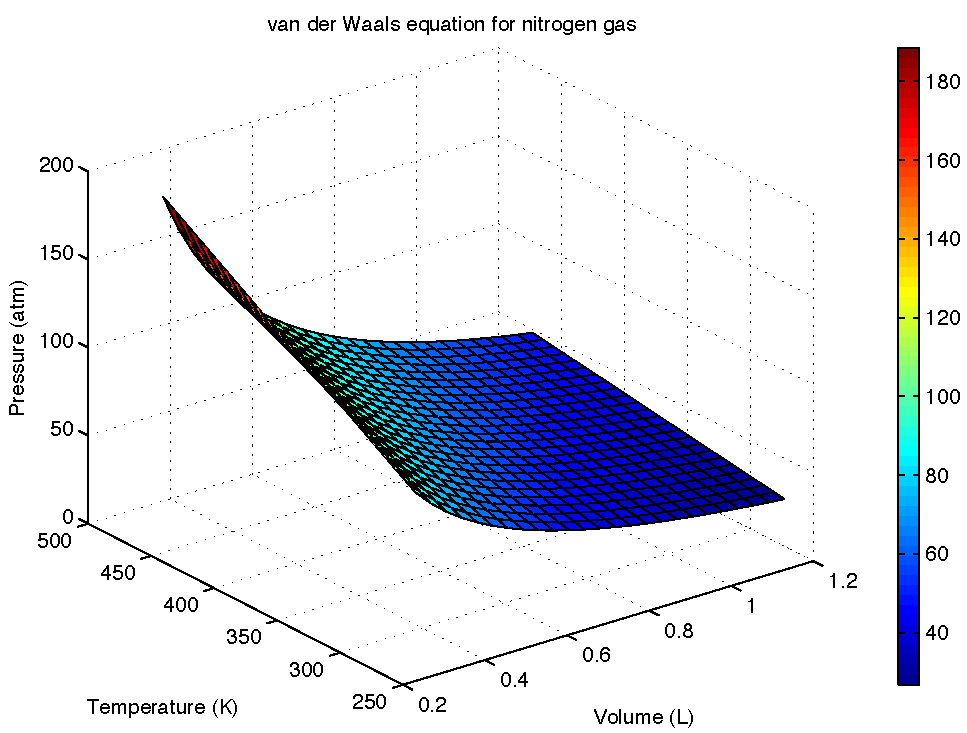
\includegraphics[width=\linewidth]{Graphics/Additional-Ex/3D-vdW-nitrogen-plot}
	\caption{van der Waals equation for nitrogen gas}
	\label{fig:3D-vdW-nitrogen-plot}
\end{figure}

\clearpage
\item
\begin{lstlisting}
>> h = 40; b = 30; yF = -15; zF = -10; F = -250000;
>> Izz = (1/12)*b*h^3;
>> Iyy = (1/12)*h*b^3;
>> A = h*b;
>> y = -h/2:h/2;
>> z = -b/2:b/2;
>> [yy, zz] = meshgrid(y,z);
>> Sxx = F/A + (F*zF*zz)./Iyy + (F*yF*yy)./Izz;
>> surf(yy,zz,Sxx), colorbar, xlabel('y (mm)'), ...
ylabel('z (mm)'), zlabel('Normal stress (N/mm^2)'), ...
title('Normal stress in a cross section of a rectangular beam')
\end{lstlisting}
\begin{figure}[h]
	\myfloatalign
	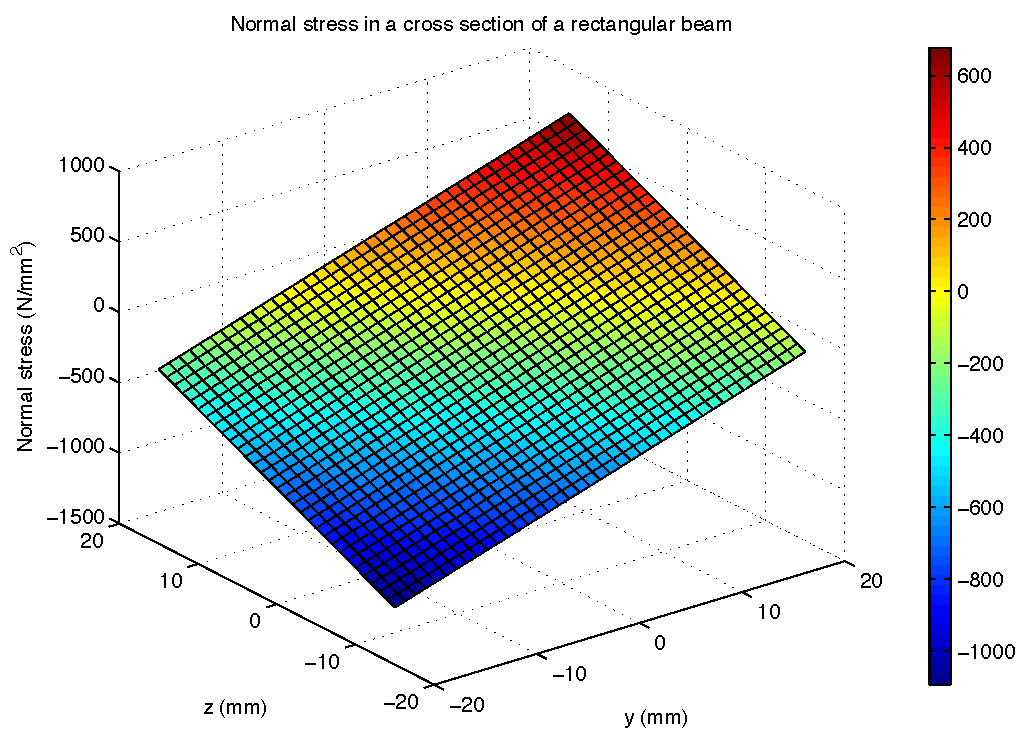
\includegraphics[width=\linewidth]{Graphics/Additional-Ex/3D-stress-plot}
	\caption{Normal stress in a cross section of a rectangular beam}
	\label{fig:3D-stress-plot}
\end{figure}

\clearpage
\item
\begin{lstlisting}
>> G = 27.7E9; b = 0.286E-9; v = 0.334;
>> x = linspace(-5E-9,5E-9,25);
>> y = linspace(-5E-9,-1E-9,25);
>> [xx, yy] = meshgrid(x,y);
>> Sxx = (-G*b*yy.*(3*xx.^2 + yy.^2)) ./ ...
(2*pi*(1-v)*(xx.^2 + yy.^2).^2);
>> Syy = (G*b*yy.*(xx.^2 - yy.^2)) ./ ...
(2*pi*(1-v)*(xx.^2 + yy.^2).^2);
>> Txy = (G*b*xx.*(xx.^2 - yy.^2)) ./ ...
(2*pi*(1-v)*(xx.^2 + yy.^2).^2);
>> figure, surf(xx,yy,Sxx), colorbar, ...
xlabel('x (m)'), ylabel('y (m)'), ...
zlabel('Normal stress Sxx (N/mm^2)'), ...
title('Stresses due to an edge dislocation in aluminium')
>> figure, surf(xx,yy,Syy), colorbar, ...
xlabel('x (m)'), ylabel('y (m)'), ...
zlabel('Normal stress Syy (N/mm^2)'), ...
title('Stresses due to an edge dislocation in aluminium')
>> figure, surf(xx,yy,Txy), colorbar, ...
xlabel('x (m)'), ylabel('y (m)'), ...
zlabel('Shear stress Txy (N/mm^2)'), ...
title('Stresses due to an edge dislocation in aluminium')
\end{lstlisting}
\begin{figure}[h]
	\myfloatalign
	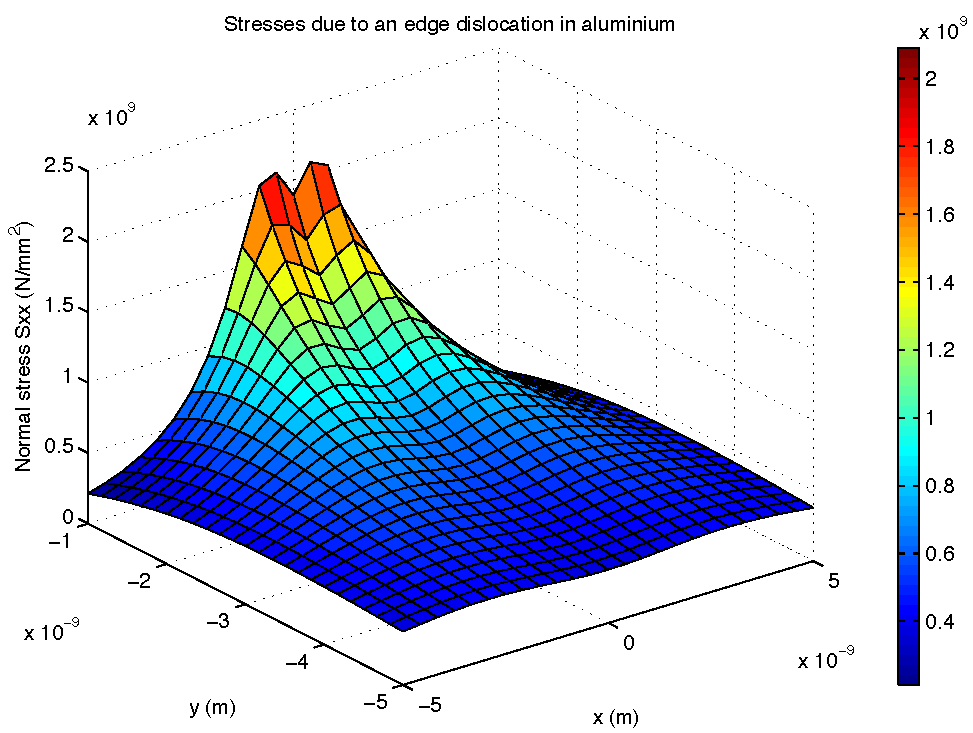
\includegraphics[width=\linewidth]{Graphics/Additional-Ex/3D-edge-disloc-plot-Sxx}
	\caption{Normal stress $\sigma_{yy}$ due to an edge dislocation in aluminium}
	\label{fig:3D-edge-disloc-plot-Sxx}
\end{figure}
\begin{figure}[h]
	\myfloatalign
	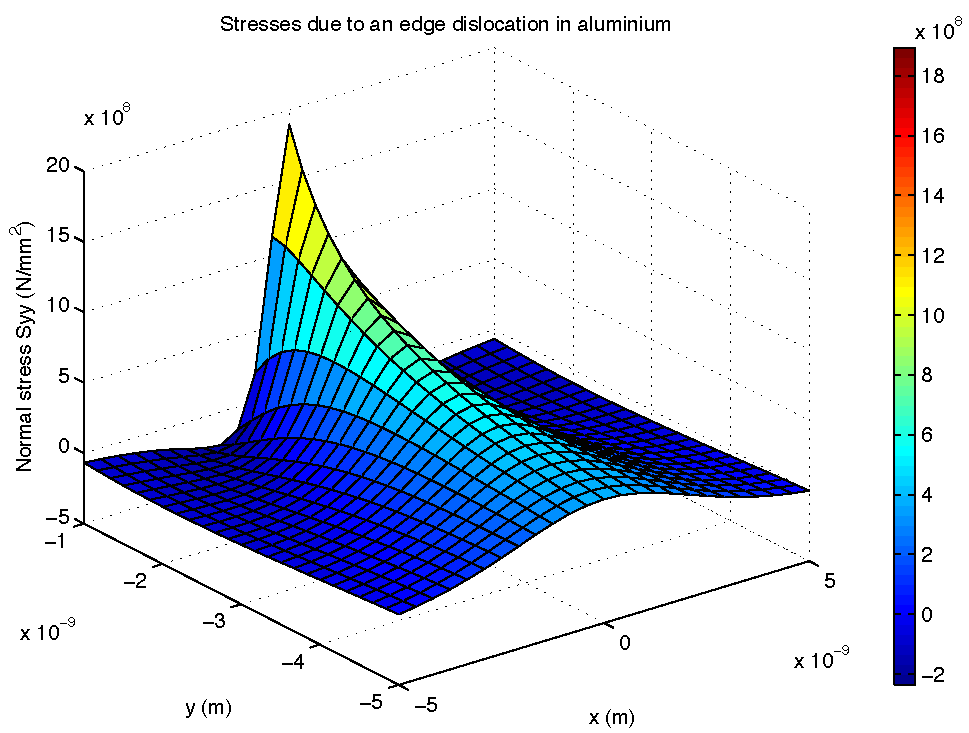
\includegraphics[width=\linewidth]{Graphics/Additional-Ex/3D-edge-disloc-plot-Syy}
	\caption{Normal stress $\sigma_{yy}$ due to an edge dislocation in aluminium}
	\label{fig:3D-edge-disloc-plot-Syy}
\end{figure}
\begin{figure}[h]
	\myfloatalign
	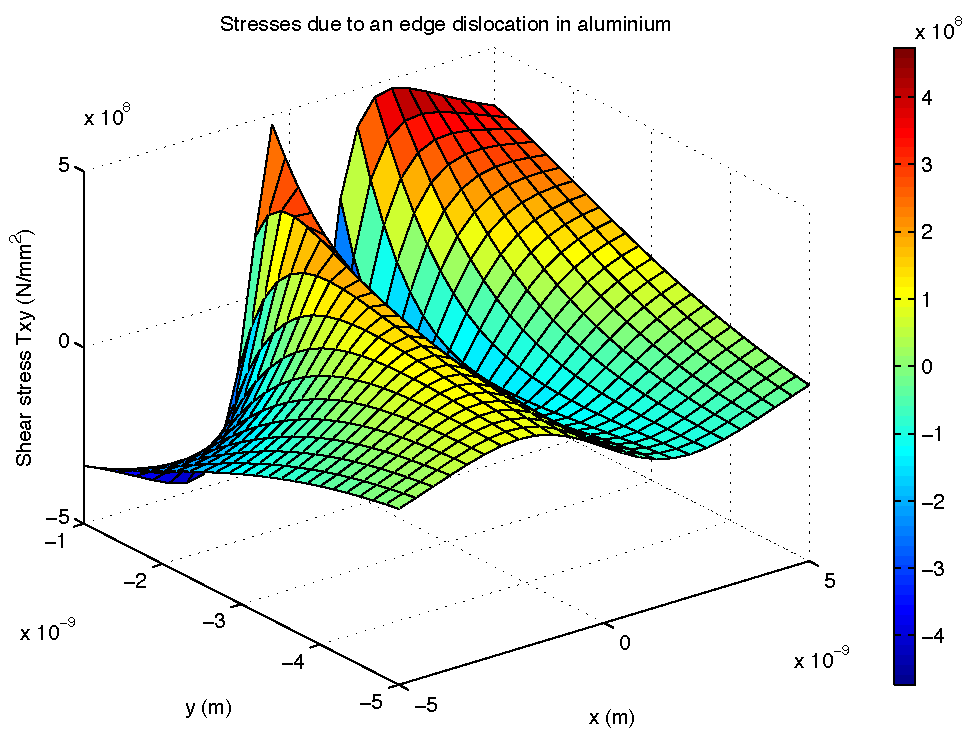
\includegraphics[width=\linewidth]{Graphics/Additional-Ex/3D-edge-disloc-plot-Txy}
	\caption{Shear stress $\tau_{xy}$ due to an edge dislocation in aluminium}
	\label{fig:3D-edge-disloc-plot-Txy}
\end{figure}

\clearpage
\item
\begin{lstlisting}
>> M = 0.032; R = 8.31;
>> v = linspace(0,1000,25);
>> T = linspace(70,320,25);
>> [vv, TT] = meshgrid(v,T);
>> P = 4*pi *(M./(2*pi*R*TT)).^(3/2) .*vv.^2 ...
*exp((-M*vv.^2)./(2*R*TT));
>> surf(vv,TT,P), colorbar, xlabel('Speed (m/s)'), ...
ylabel('Temperature (K)'), zlabel('Probability'), ...
title('Probability distribution of speeds of molecules ... 
of oxygen gas')
\end{lstlisting}
\begin{figure}[h]
	\myfloatalign
	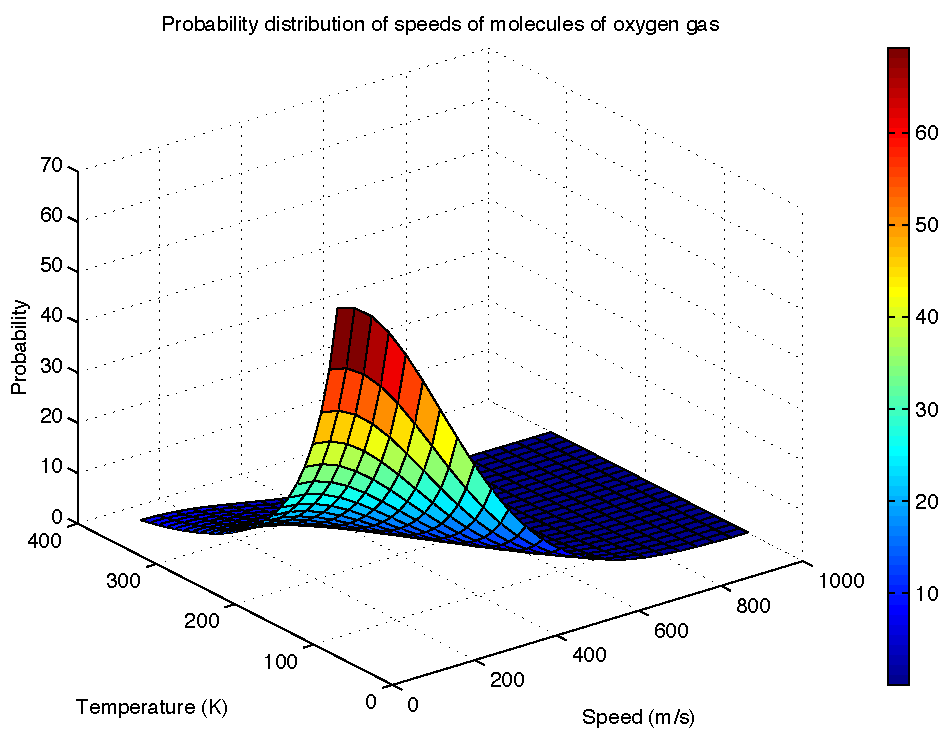
\includegraphics[width=\linewidth]{Graphics/Additional-Ex/3D-oxygen-plot}
	\caption{Probability distribution of speeds of molecules of oxygen gas}
	\label{fig:3D-oxygen-plot}
\end{figure}

\clearpage
\item
\begin{lstlisting}
>> C = 15E-6; L = 240E-3; vm = 24;
>> fd = linspace(60,110,25);
>> R = linspace(10,40,25);
>> wd = 2*pi*fd;
>> [ww, RR] = meshgrid(wd,R);
>> I = vm ./ (sqrt(RR^2 + (ww*L - 1./(ww*C)).^2));
>> surf(ww,RR,I), colorbar, xlabel('Frequency (rads)'), ...
ylabel('Resistance (Ohms)'), zlabel('Current (A)'), ...
title('Current in an RLC circuit with alternating ...
voltage source')
\end{lstlisting}
\begin{figure}[h]
	\myfloatalign
	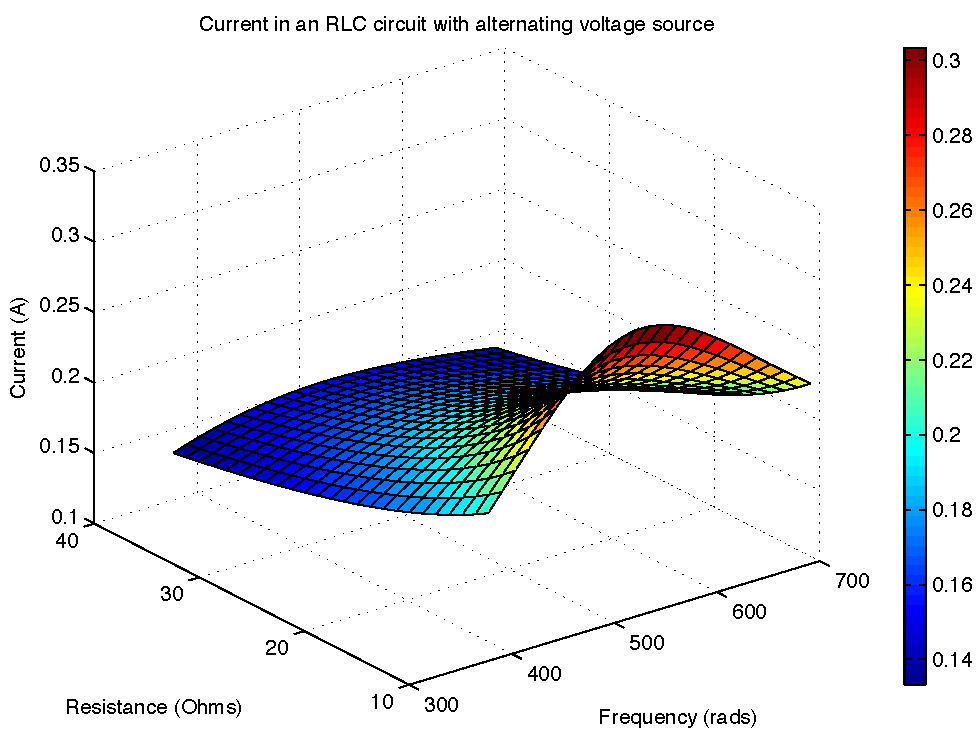
\includegraphics[width=\linewidth]{Graphics/Additional-Ex/3D-RLC-plot}
	\caption{Current in an \textit{RLC} circuit with alternating voltage source}
	\label{fig:3D-RLC-plot}
\end{figure}
\begin{figure}[h]
	\myfloatalign
	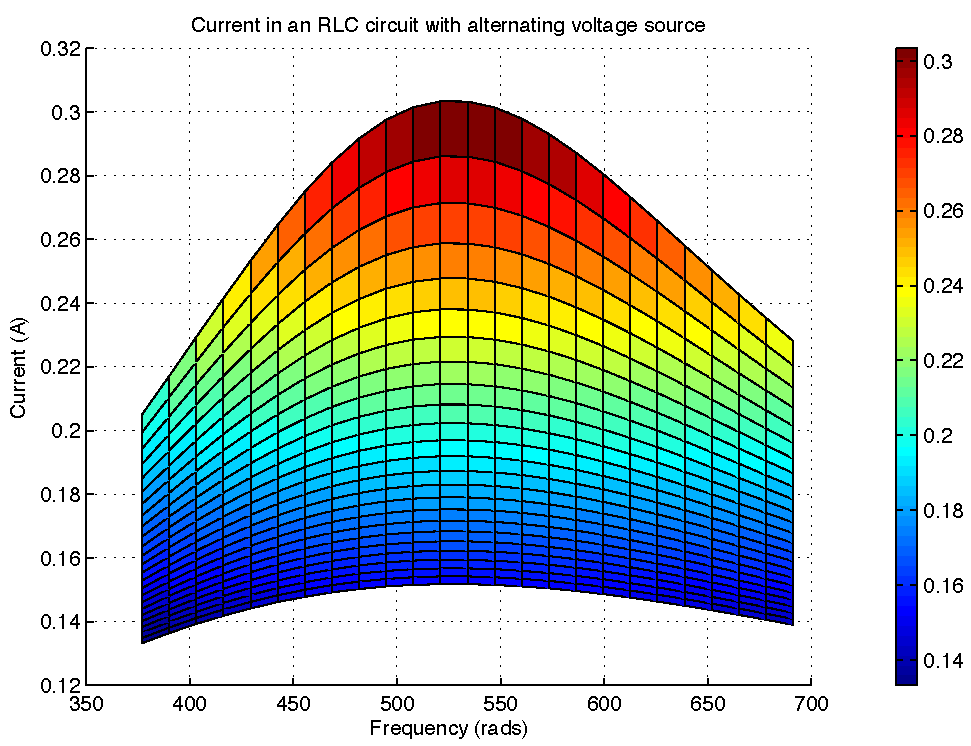
\includegraphics[width=\linewidth]{Graphics/Additional-Ex/3D-RLC-plot-rotate}
	\caption{Current in an \textit{RLC} circuit with alternating voltage source}
	\label{fig:3D-RLC-plot-rotate}
\end{figure}
Examining Figure~\ref{fig:3D-RLC-plot-rotate} shows the maximum current occurs at approximately $525~rads/2\pi=84~Hz$. This compares well with the calculated value:
\begin{equation*}
\frac{1}{2\pi\sqrt{LC}} = 83.882~Hz
\end{equation*}

\clearpage
\section*{Scripts and Functions}
\item \lstinputlisting[caption={\textit{silo.m} - Script to calculate the height and surface area of a spherical capped cylindrical silo},label=lst:silo]{MATLAB-code/Additional-Ex/silo.m}

\newpage
\item Calculate the decay constant $k$ for Technetium-99.
\begin{align*}
& \frac{A_0}{2} = A_0 e^{6k}, \\
& \Leftrightarrow ln \left( \frac{A_0}{2} \right) = ln \left( A_0 e^{6k} \right) \\
& \Leftrightarrow ln \left( \frac{A_0}{2} \right) = ln (A_0) + ln \left( e^{6k} \right) \\
& \Leftrightarrow 6k = ln \left( \frac{A_0}{2} \right) - ln(A_0) \\
& \Leftrightarrow 6k = ln \left( \frac{A_0}{2} \frac{1}{A_0}\right)  \\
& \Leftrightarrow 6k = ln (0.5)  \\
& \Leftrightarrow k = -0.1155
\end{align*}
\lstinputlisting[caption={\textit{decay.m} - Script to calculate the radioactive decay of Technetium-99},label=lst:decay]{MATLAB-code/Additional-Ex/decay.m}
\begin{figure}[h]
	\myfloatalign
	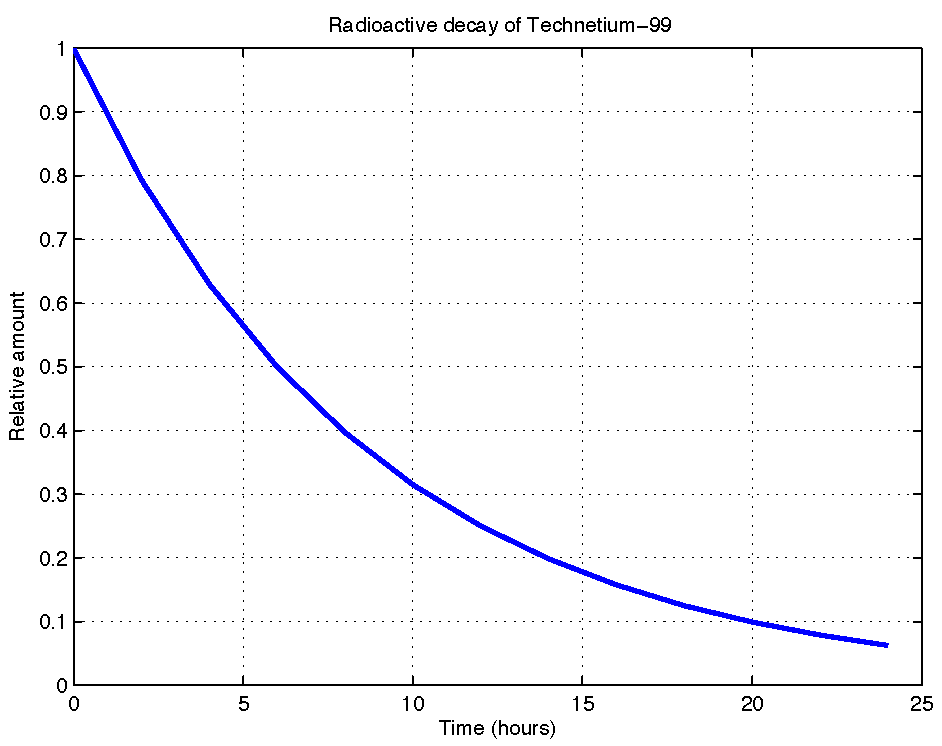
\includegraphics[width=\linewidth]{Graphics/Additional-Ex/decay-plot}
	\caption{Radioactive decay of Technetium-99}
	\label{fig:decay-plot}
\end{figure}

\clearpage
\item \lstinputlisting[caption={\textit{benzene.m} - Script to calculate the pressure of Benzene},label=lst:benzene]{MATLAB-code/Additional-Ex/benzene.m}
\begin{figure}[h]
	\myfloatalign
	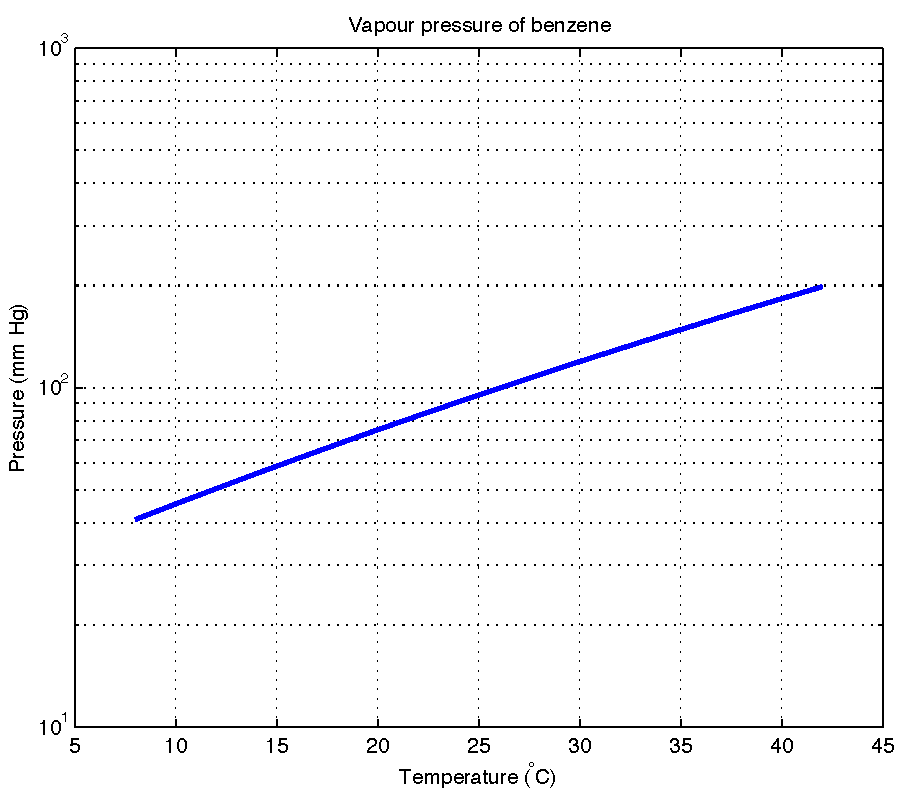
\includegraphics[width=0.9\linewidth]{Graphics/Additional-Ex/benzene}
	\caption{Vapour pressure of benzene}
	\label{fig:benzene}
\end{figure}

\newpage
\item \lstinputlisting[caption={\textit{cubic\_gases.m} - Script to calculate heat capacity for 4 gases},label=lst:cubic_gases]{MATLAB-code/Additional-Ex/cubic_gases.m}

\newpage
\item \lstinputlisting[caption={\textit{trajectory.m} - Function to calculate the trajectory of a projectile},label=lst:trajectory]{MATLAB-code/Additional-Ex/trajectory.m}
\begin{figure}[h]
	\myfloatalign
	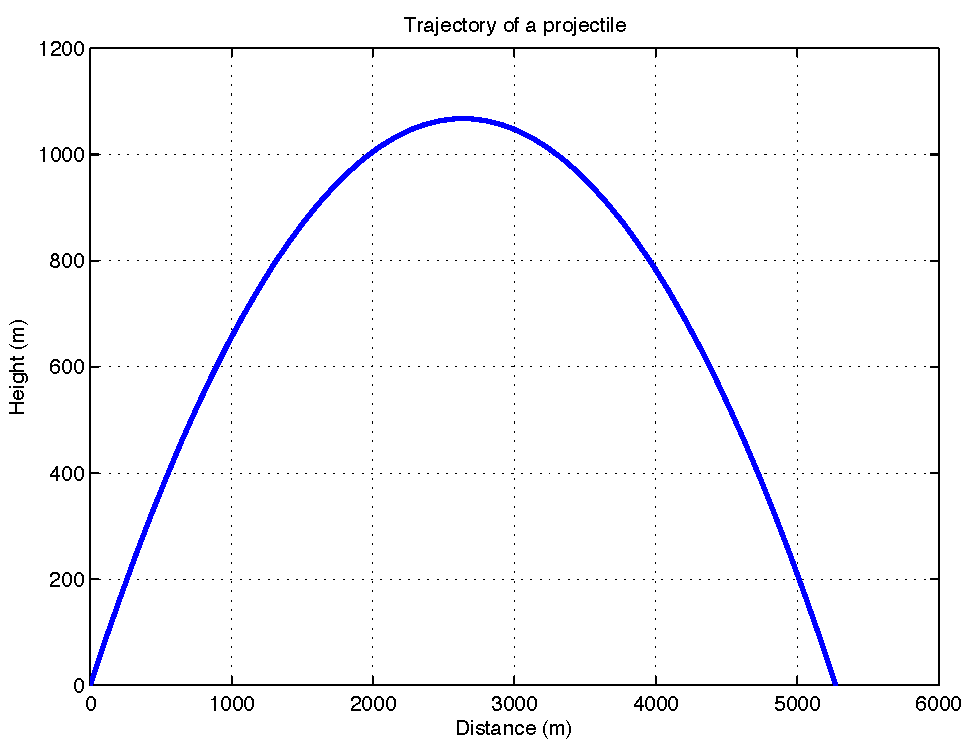
\includegraphics[width=\linewidth]{Graphics/Additional-Ex/trajectory}
	\caption{Trajectory of a projectile}
	\label{fig:trajectory}
\end{figure}

\newpage
\item \lstinputlisting[caption={\textit{STtoSI.m} - Function to convert height and mass in imperial units to metric},label=lst:STtoSI]{MATLAB-code/Additional-Ex/STtoSI.m}
Running the function in the Command Window with the example:
\begin{lstlisting}
>> [m, kg] = STtoSI(((5*12)+11),181)
m = 
    1.8034
kg = 
   82.0862
\end{lstlisting}

\newpage
\item \lstinputlisting[caption={\textit{req.m} - Function to calculate resistance of resistors in parallel},label=lst:req]{MATLAB-code/Additional-Ex/req.m}
Running the function in the Command Window with the example:
\begin{lstlisting}
>> REQ = req([50 75 300 60 500 180 200]
REQ = 
      15.1771
\end{lstlisting}

\item \lstinputlisting[caption={\textit{princstress.m} - Function to calculate principal stresses from stress components},label=lst:princstress]{MATLAB-code/Additional-Ex/princstress.m}
Running the function in the Command Window with the example:
\begin{lstlisting}
>> [Smax, Smin] = princstress(-190,145,110)
Smax = 
       177.8902
Smin = 
      -222.8902
\end{lstlisting}

\newpage
\item \lstinputlisting[caption={\textit{lowpass.m} - Function to calculate magnitude ratio of a lowpass filter},label=lst:lowpass]{MATLAB-code/Additional-Ex/lowpass.m}
\lstinputlisting[caption={\textit{lowpass\_plot.m} - Script to plot the magnitude ratio of a lowpass filter},label=lst:lowpass_plot]{MATLAB-code/Additional-Ex/lowpass_plot.m}
\begin{figure}[h]
	\myfloatalign
	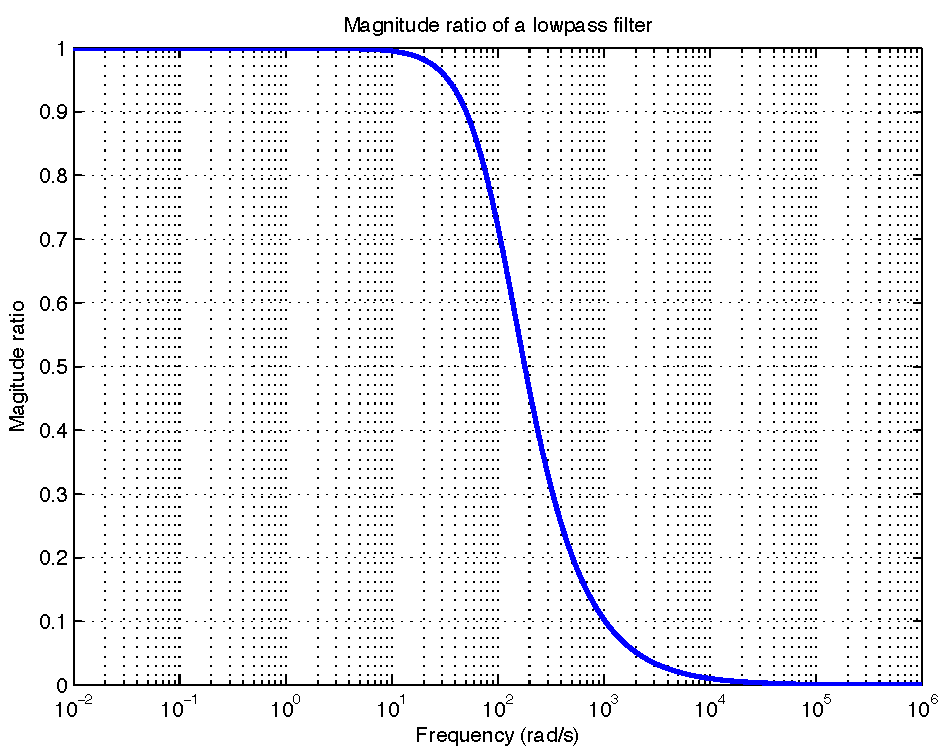
\includegraphics[width=\linewidth]{Graphics/Additional-Ex/lowpass-plot}
	\caption{Magnitude ratio of a lowpass filter}
	\label{fig:lowpass-plot}
\end{figure}

\clearpage
\section*{Decision Making}
\item \lstinputlisting[caption={\textit{temp.m} - Script to analyse temperature data},label=lst:temp]{MATLAB-code/Additional-Ex/temp.m}

%\newpage
%\item \lstinputlisting[caption={\textit{drugA.m} - Script to calculate and plot concentration of drugs in the human body},label=lst:drugA]{MATLAB-code/Additional-Ex/drugA.m}
%\begin{figure}[h]
%	\myfloatalign
%	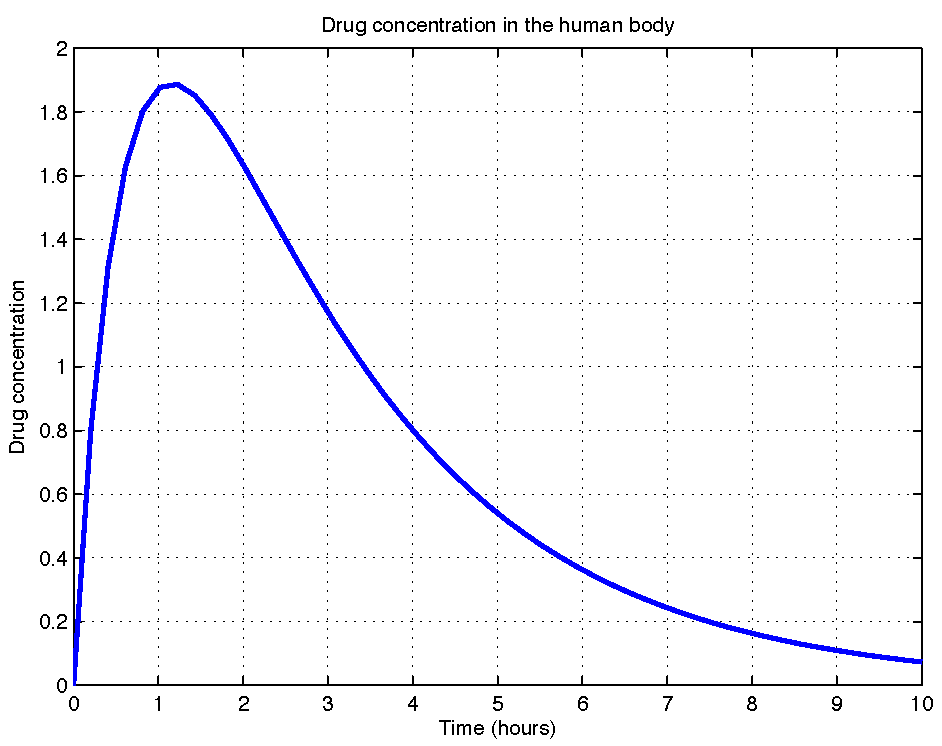
\includegraphics[width=\linewidth]{Graphics/Additional-Ex/drugA}
%	\caption{Concentration of drugs in the human body}
%	\label{fig:drugA}
%\end{figure}

%\clearpage
\section*{Loops}
%\item \lstinputlisting[caption={\textit{drugB.m} - Script to calculate and plot concentration of drugs in the human body},label=lst:drugB]{MATLAB-code/Additional-Ex/drugB.m}
%\begin{figure}[h]
%	\myfloatalign
%	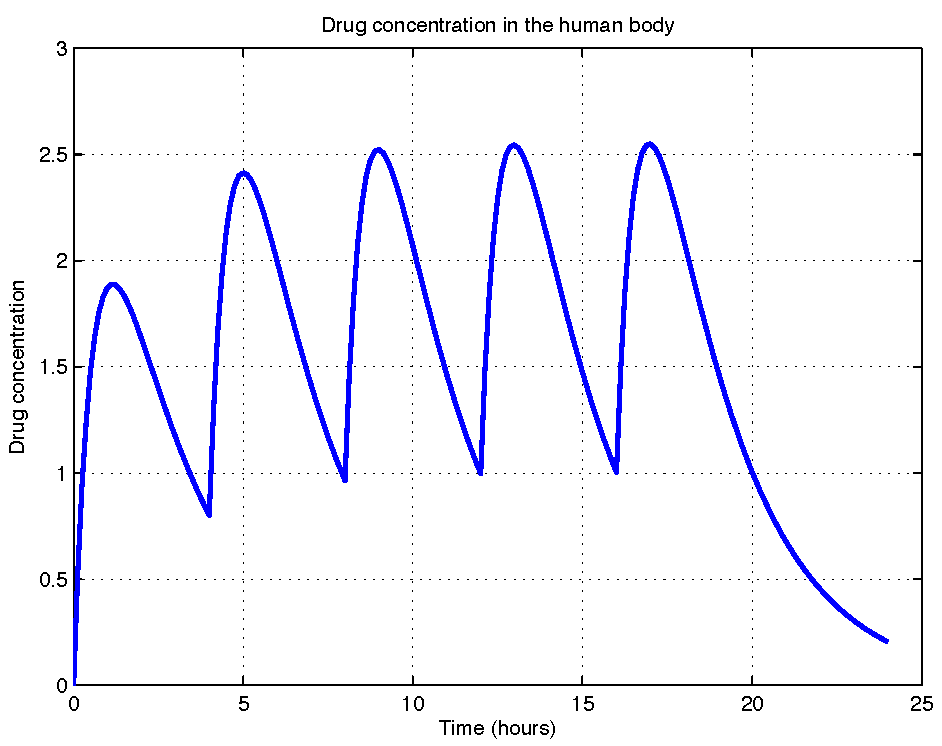
\includegraphics[width=\linewidth]{Graphics/Additional-Ex/drugB}
%	\caption{Concentration of drugs in the human body}
%	\label{fig:drugB}
%\end{figure}

\clearpage
\item \lstinputlisting[caption={\textit{rocket.m} - Script to calculate and plot the speed and altitude of a rocket},label=lst:rocket]{MATLAB-code/Additional-Ex/rocket.m}
\begin{figure}[h]
	\myfloatalign
	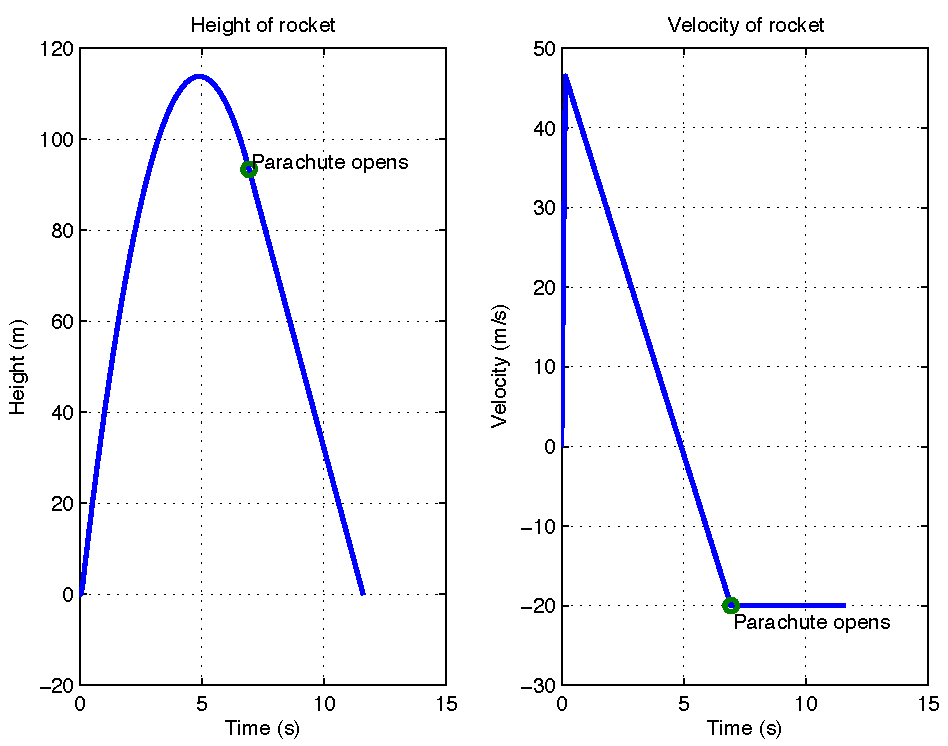
\includegraphics[width=\linewidth]{Graphics/Additional-Ex/rocket-plot}
	\caption{Speed and altitude of a rocket}
	\label{fig:rocket-plot}
\end{figure}

\end{enumerate}
